\documentclass[11pt,a4paper]{article}
\usepackage[margin=2cm]{geometry}
\usepackage[T1]{fontenc}
\usepackage{lmodern}
\usepackage{microtype}
\usepackage{booktabs}
\usepackage{tabularx}
\usepackage{float}
\usepackage{xcolor}
\usepackage{tikz}
\usetikzlibrary{fit,arrows.meta,backgrounds,positioning}
\usepackage[font=small,skip=8pt]{caption}
\usepackage{enumitem}
\usepackage{titlesec}
\usepackage{xurl}
\usepackage[hidelinks]{hyperref}

\setlist{nosep,leftmargin=1.2em}
\setlength{\parskip}{0.4em}
\setlength{\parindent}{0pt}
\titlespacing*{\section}{0pt}{0.9em}{0.5em}
\titleformat*{\section}{\large\bfseries}
\setlength{\textfloatsep}{12pt plus 2pt}
\setlength{\floatsep}{10pt plus 2pt}
\renewcommand{\topfraction}{0.9}
\renewcommand{\floatpagefraction}{0.8}
\DeclareUrlCommand\code{\urlstyle{tt}}
\newcommand{\choice}[1]{\par\smallskip\textbf{#1}\enspace}
% A path in the repository, linked to its page on GitHub.
\newcommand{\repo}[1]{\href{https://github.com/kkkamur07/nomikos/tree/main/#1}{\code{#1}}}

\definecolor{accent}{HTML}{B40000}
\definecolor{boxfill}{HTML}{F6F3EE}
\definecolor{groupline}{HTML}{8A8378}

\tikzset{
  box/.style={draw, rounded corners=2pt, fill=boxfill, align=center,
    inner xsep=6pt, inner ysep=4pt, minimum width=2.5cm, minimum height=0.85cm,
    font=\footnotesize},
  store/.style={box, fill=white},
  group/.style={draw=groupline, dashed, rounded corners=6pt, inner sep=8pt},
  glabel/.style={font=\scriptsize\itshape, text=groupline, anchor=south west, inner sep=2pt},
  run/.style={-{Stealth[length=5pt]}, thick},
  art/.style={-{Stealth[length=5pt]}, thick, dashed},
  lab/.style={font=\scriptsize, fill=white, inner sep=1.5pt, align=center},
  key/.style={font=\scriptsize, anchor=west},
}

\begin{document}

{\LARGE\bfseries Nomikos: Advanced Programming report}\par
\smallskip
{\large Krrish Agarwalla and Astha Gupta}\par
\smallskip
{\small Live at \href{https://nomikos.app}{\texttt{nomikos.app}}, code at \href{https://github.com/kkkamur07/nomikos}{\texttt{github.com/kkkamur07/nomikos}}.}

Nomikos is a web platform for handwritten text recognition of Byzantine Greek, Armenian, Syriac and Coptic manuscripts. A researcher uploads page images and runs a segmenter, which finds the lines on a page, and a recogniser, which reads each line. They fix the output in a browser editor and export PAGE XML (a standard format for page layout and text), docx, PDF or plain text.

We built Nomikos around two goals.
\begin{enumerate}
  \item \textbf{Researchers verify, they do not transcribe.} The models and the platform do the heavy lifting: they find the lines on a page and read them. The researcher checks the result and fixes what is wrong. Our target is to make transcription ten times faster than typing it by hand. Every fix is stored apart from the model's guess (Section~\ref{sec:data}), so it becomes training data for the next model.
  \item \textbf{Models in the researcher's workflow, without the setup.} Running a research model usually means a GPU, a Python environment and the authors' training code. On Nomikos a researcher uploads pages in the browser, picks a model and gets the output, with nothing to install. Jobs run on our hosted runner, or on the researcher's own computer, where the compute costs us nothing.
\end{enumerate}

Existing HTR platforms did not fit these goals. eScriptorium is open source but built around one engine, kraken, and someone has to host an instance. Transkribus lets users train and apply their own models, but only inside its own cloud, where recognition is metered in credits.

\section{System overview}

Figure~\ref{fig:containers} shows two paths.

On the request path, the browser loads the editor from Vercel once and from then on sends every call to the FastAPI API, the only backend service that accepts incoming HTTP. The API holds all business logic. It reads and writes Postgres, keeps page images in a media directory on the host, and streams job updates back to the browser as server-sent events (SSE), a one-way stream over an ordinary HTTP connection.

On the work path, models run in the \emph{inference runner}, a small Python program published on PyPI. The researcher chooses where a job runs: locally, on a runner installed on their own computer with one command, or in the cloud, on the runner we host, which needs no install. Both are the same program. A runner asks the API for a job, downloads the page image, runs the model and posts the result back. GitHub Actions publishes each runner release to PyPI, and the runner fetches model weights from the Hugging Face Hub. A separate platform worker handles jobs that need no model, such as building exports, and reads the same media directory without write access.

\begin{figure}[!ht]
\centering
\resizebox{0.88\linewidth}{!}{%
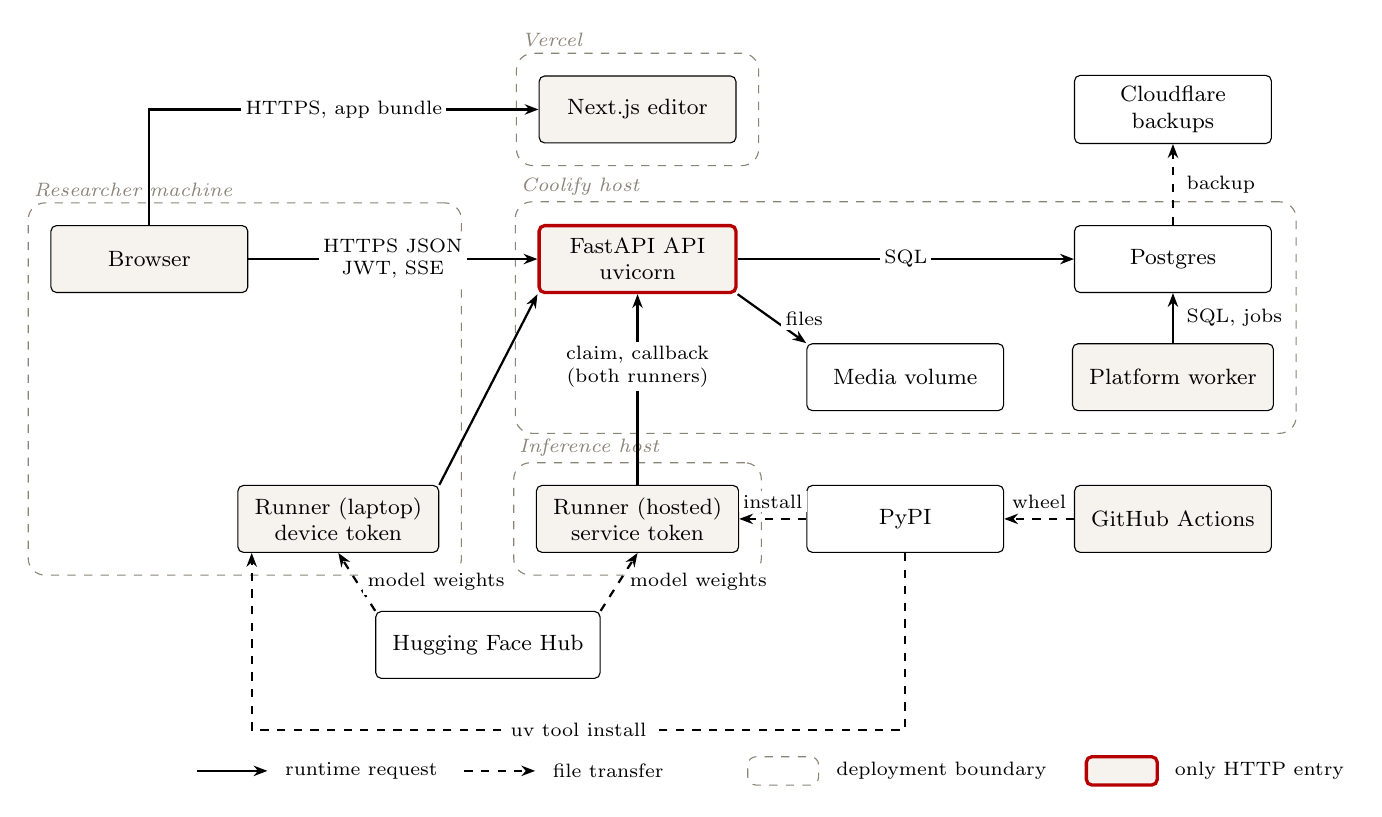
\begin{tikzpicture}
  \node[box] (browser) at (0,0) {Browser};
  \node[box] (laptop) at (2.4,-3.3) {Runner (laptop)\\device token};
  \node[box] (next) at (6.2,1.9) {Next.js editor};
  \node[box, draw=accent, very thick] (api) at (6.2,0) {FastAPI API\\uvicorn};
  \node[store] (pg) at (13.0,0) {Postgres};
  \node[store] (cf) at (13.0,1.9) {Cloudflare\\backups};
  \node[store] (media) at (9.6,-1.5) {Media volume};
  \node[box] (worker) at (13.0,-1.5) {Platform worker};
  \node[box] (hosted) at (6.2,-3.3) {Runner (hosted)\\service token};
  \node[store] (hf) at (4.3,-4.9) {Hugging Face Hub};
  \node[store] (pypi) at (9.6,-3.3) {PyPI};
  \node[box] (gha) at (13.0,-3.3) {GitHub Actions};

  \begin{scope}[on background layer]
    \node[group, fit=(browser)(laptop)] (gres) {};
    \node[group, fit=(next)] (gvercel) {};
    \node[group, fit=(api)(pg)(media)(worker)] (gcool) {};
    \node[group, fit=(hosted)] (ginf) {};
  \end{scope}
  \node[glabel] at (gres.north west) {Researcher machine};
  \node[glabel] at (gvercel.north west) {Vercel};
  \node[glabel] at (gcool.north west) {Coolify host};
  \node[glabel] at (ginf.north west) {Inference host};

  \draw[run] (browser.north) |- node[lab, pos=0.75] {HTTPS, app bundle} (next.west);
  \draw[run] (browser) -- node[lab] {HTTPS JSON\\JWT, SSE} (api);
  \draw[run] (api) -- node[lab] {SQL} (pg);
  \draw[run] (api.south east) -- node[lab, right=3pt] {files} (media.north west);
  \draw[run] (worker) -- node[lab, right=3pt] {SQL, jobs} (pg);
  \draw[run] (laptop.north east) -- (api.south west);
  \draw[run] (hosted) -- node[lab, pos=0.62] {claim, callback\\(both runners)} (api);
  \draw[art] (hf.north west) -- node[lab, right=2pt] {model weights} (laptop.south);
  \draw[art] (hf.north east) -- node[lab, right=2pt] {model weights} (hosted.south);
  \draw[art] (pypi) -- node[lab, above=2pt] {install} (hosted);
  \draw[art] (pypi.south) |- ++(0,-2.25) -| node[lab, pos=0.25] {uv tool install} ([xshift=-11mm]laptop.south);
  \draw[art] (gha) -- node[lab, above=2pt] {wheel} (pypi);
  \draw[art] (pg) -- node[lab, right=3pt] {backup} (cf);

  \begin{scope}[shift={(0.6,-6.5)}]
    \draw[run] (0,0) -- (0.9,0); \node[key] at (1.0,0) {runtime request};
    \draw[art] (3.4,0) -- (4.3,0); \node[key] at (4.4,0) {file transfer};
    \draw[groupline, dashed, rounded corners=3pt] (7.0,-0.18) rectangle (7.9,0.18);
    \node[key] at (8.0,0) {deployment boundary};
    \draw[accent, very thick, rounded corners=2pt, fill=boxfill] (11.3,-0.18) rectangle (12.2,0.18);
    \node[key] at (12.3,0) {only HTTP entry};
  \end{scope}
\end{tikzpicture}}
\caption{Containers and where they run. The browser loads the editor from Vercel and then talks to the API directly. Both runners are the same PyPI package and only make outbound calls.}
\label{fig:containers}
\end{figure}

All stateful parts sit on one Coolify host: the API container, the Postgres container, the media directory and the platform worker. Postgres is backed up off the host to Cloudflare. The hosted runner lives on a separate machine as systemd units.

\choice{Frontend on Vercel, backend on Coolify.} Vercel builds and serves Next.js natively and caches it on a global edge network, so the editor loads fast. The backend needs what serverless platforms handle poorly: a long-running worker, a direct database connection, a disk for images and connections that stay open for the SSE streams (Section~\ref{sec:jobs}). Coolify deploys our containers from Git on our own server, and we take care of that server, its releases and its backups.

The frontend runs entirely in the browser. TanStack Query caches every API response for 30 seconds and refetches when the tab regains focus or the network comes back. In the editor, a line's text is saved when the line loses focus, edits can be undone, and saved states of a page go into a history the user can restore from. While a job runs, all components that care about it share one event stream for that job, and if no event arrives for 12 seconds the browser falls back to polling.

We chose tools with broad support that we already knew (Table~\ref{tab:stack}).

\begin{table}[ht]
\centering
\small
\begin{tabularx}{0.95\linewidth}{@{}l l >{\raggedright\arraybackslash}X@{}}
\toprule
Layer & Choice & Functionality \\
\midrule
Frontend & \href{https://nextjs.org}{Next.js 16}, React 19, TypeScript & The web app researchers use: upload pages, check and correct the model output, export the result \\
API & \href{https://fastapi.tiangolo.com}{FastAPI}, SQLAlchemy 2 (async) & The server behind the app: answers every request, checks who may see and change what, and holds all business logic \\
Database & \href{https://www.postgresql.org}{PostgreSQL 16}, \href{https://alembic.sqlalchemy.org}{Alembic} & Stores all data and also serves as the job queue; Alembic keeps the revision history of the schema \\
Inference & \href{https://onnxruntime.ai}{ONNX Runtime} on CPU & Runs the machine learning models that find lines and read text, on an ordinary computer without a GPU \\
Models & \href{https://huggingface.co/nomikos-project}{Hugging Face Hub} & Stores the trained model files, each pinned to an exact version; our models and datasets are public there \\
Hosting & \href{https://vercel.com}{Vercel}, \href{https://coolify.io}{Coolify} & Puts the system online: Vercel serves the web app, Coolify runs the server and database on our machine \\
Backups & \href{https://www.cloudflare.com}{Cloudflare} & Keeps copies of the data away from our server \\
CI & GitHub Actions & Checks and tests every change automatically and publishes new releases \\
\bottomrule
\end{tabularx}
\caption{The stack. The Python inference runner is published on PyPI as \href{https://pypi.org/project/nomikos-inference/}{\texttt{nomikos-inference}}.}
\label{tab:stack}
\end{table}

\section{Job flow}\label{sec:jobs}

\begin{figure}[!ht]
\centering
\resizebox{0.8\linewidth}{!}{%
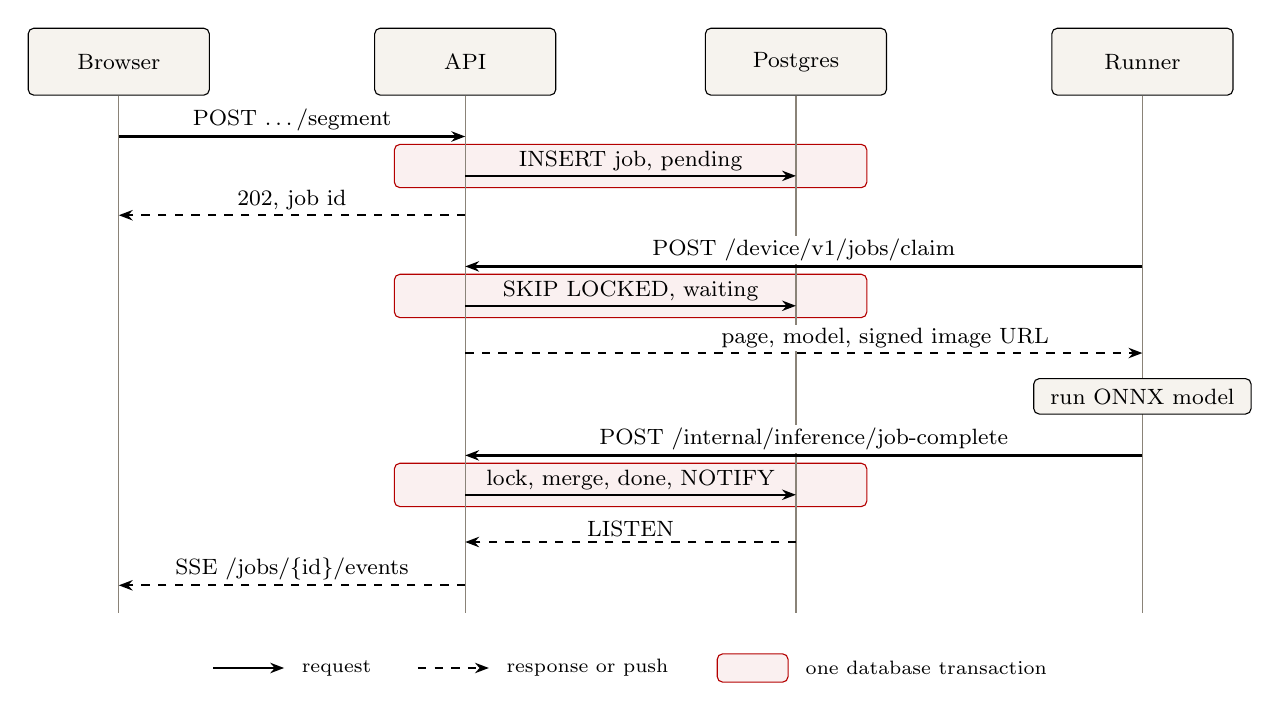
\begin{tikzpicture}[
  actor/.style={box, minimum width=2.3cm},
  msg/.style={-{Stealth[length=5pt]}, thick},
  ret/.style={-{Stealth[length=5pt]}, thick, dashed},
  ml/.style={font=\footnotesize, above=0.5pt, inner sep=1pt, fill=white},
  tx/.style={draw=accent, fill=accent!6, rounded corners=2pt}]
  \def\xb{0} \def\xa{4.4} \def\xd{8.6} \def\xg{13.0}
  % transaction bands behind each POST, wide enough to hold their labels
  \begin{scope}[on background layer]
    \fill[tx] (\xa-0.9,-1.6) rectangle (\xd+0.9,-1.05);
    \fill[tx] (\xa-0.9,-3.25) rectangle (\xd+0.9,-2.7);
    \fill[tx] (\xa-0.9,-5.65) rectangle (\xd+0.9,-5.1);
  \end{scope}
  \foreach \x/\n in {\xb/Browser, \xa/API, \xd/Postgres, \xg/Runner} {
    \node[actor] at (\x,0) {\n};
    \draw[groupline] (\x,-0.43) -- (\x,-7.0);
  }
  \draw[msg] (\xb,-0.95) -- node[ml] {POST \dots/segment} (\xa,-0.95);
  \draw[msg] (\xa,-1.45) -- node[ml, fill=none] {INSERT job, pending} (\xd,-1.45);
  \draw[ret] (\xa,-1.95) -- node[ml] {202, job id} (\xb,-1.95);
  \draw[msg] (\xg,-2.6) -- node[ml] {POST /device/v1/jobs/claim} (\xa,-2.6);
  \draw[msg] (\xa,-3.1) -- node[ml, fill=none] {SKIP LOCKED, waiting} (\xd,-3.1);
  \draw[ret] (\xa,-3.7) -- node[ml, pos=0.62] {page, model, signed image URL} (\xg,-3.7);
  \node[box, minimum width=2.1cm, minimum height=0.45cm, inner ysep=1pt] at (\xg,-4.25) {run ONNX model};
  \draw[msg] (\xg,-5.0) -- node[ml] {POST /internal/inference/job-complete} (\xa,-5.0);
  \draw[msg] (\xa,-5.5) -- node[ml, fill=none] {lock, merge, done, NOTIFY} (\xd,-5.5);
  \draw[ret] (\xd,-6.1) -- node[ml] {LISTEN} (\xa,-6.1);
  \draw[ret] (\xa,-6.65) -- node[ml] {SSE /jobs/\{id\}/events} (\xb,-6.65);
  \begin{scope}[shift={(1.2,-7.7)}]
    \draw[msg] (0,0) -- (0.9,0); \node[key] at (1.0,0) {request};
    \draw[ret] (2.6,0) -- (3.5,0); \node[key] at (3.6,0) {response or push};
    \fill[tx] (6.4,-0.18) rectangle (7.3,0.18); \node[key] at (7.4,0) {one database transaction};
  \end{scope}
\end{tikzpicture}}
\caption{One segmentation job. Each of the three POST requests is a single transaction; the browser hears about the result through \texttt{NOTIFY} and server-sent events.}
\label{fig:jobs}
\end{figure}

A job is one page and one model, and Figure~\ref{fig:jobs} follows it. Three POST requests drive it, and each one is a single database transaction, so a crash leaves the job in a known state. The browser's POST inserts a \texttt{pending} row and returns at once. A runner's claim POST locks one pending row, skipping rows other runners hold, and marks it \texttt{waiting}. The runner fetches the image through a signed URL, runs the model locally and sends the result in the completion POST. That handler locks the job, sets \code{callback_claimed_at} so a retried callback cannot merge twice, writes the run and the lines, marks the job \texttt{done} and fires \texttt{NOTIFY}, which wakes every process listening on that Postgres channel. Each API process keeps one \texttt{LISTEN} connection that feeds all its open streams, and it pushes the result to the browser over the job's SSE stream at \texttt{/jobs/\{id\}/events}. If the stream is blocked, the browser polls \texttt{GET /jobs/\{id\}}. A runner reports a heartbeat while it works. If the heartbeats stop, its lease expires and the job goes back to \texttt{pending}; after five expired leases the job is marked failed.

\section{Design decisions}

\choice{One process, six contexts.} The API is one process split into six bounded contexts (users, project, document, annotation, ml, jobs), each with \code{api}, \code{application}, \code{domain} and \code{infrastructure} layers. Microservices would add network hops, several databases and distributed transactions. A monolith gives one deploy and one transaction per request, and one schema whose revisions Alembic records. The price is that boundaries are only conventions: document, annotation, ml and jobs import each other in both directions.

\choice{Postgres is the queue.} The \code{jobs} table is the only queue. We did not add Redis or RabbitMQ, so a job and the data it writes commit in the same transaction and nothing can drift between two stores. Runners pull work with \texttt{SELECT \dots\ FOR UPDATE SKIP LOCKED}, which lets many workers claim rows without blocking each other. The cost is that Postgres carries the queue load on top of every other request.

\choice{Runners connect outward.} Only the token tells the two runners apart (Figure~\ref{fig:security}). A device token claims its owner's local jobs, a service token claims cloud jobs. This splits the compute bill. A local job runs on the researcher's own machine and costs us nothing; a cloud job runs on our host, which is the only inference we pay for. The hosted runner serves anyone without a capable laptop or who does not want to install anything. Because the runner always opens the connection, it works behind a university firewall without port forwarding, and the server never needs to know where runners are. The alternative, a server that pushes work to a listening inference service, needs open ports, a registry of worker addresses and a second code path. The cost is that runners stop whenever the API is down.

\choice{ONNX Runtime serves, PyTorch only exports.} The runner lives on researchers' laptops, some with only 8\,GB of memory, so we chose \href{https://onnxruntime.ai}{ONNX Runtime} because it is light. Figure~\ref{fig:onnxbars} compares it with PyTorch for serving.

\begin{figure}[!ht]
\centering
\resizebox{0.62\linewidth}{!}{%
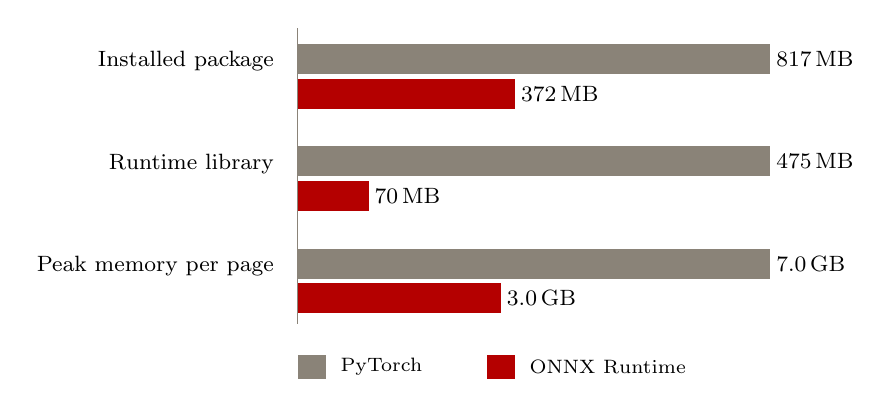
\begin{tikzpicture}[x=0.06cm, bl/.style={font=\footnotesize, anchor=west, inner sep=2pt}]
  \definecolor{torchc}{HTML}{8A8378}
  \foreach \y/\name/\pt/\ox/\tl/\ol in {
      0/Installed package/100/46/817\,MB/372\,MB,
      -1.3/Runtime library/100/15/475\,MB/70\,MB,
      -2.6/Peak memory per page/100/43/7.0\,GB/3.0\,GB} {
    \node[font=\footnotesize, anchor=east] at (-3,\y-0.22) {\name};
    \fill[torchc] (0,\y) rectangle (\pt,\y-0.38);
    \node[bl] at (\pt,\y-0.19) {\tl};
    \fill[accent] (0,\y-0.44) rectangle (\ox,\y-0.82);
    \node[bl] at (\ox,\y-0.63) {\ol};
  }
  \draw[groupline] (0,0.2) -- (0,-3.55);
  \begin{scope}[shift={(0,-4.1)}]
    \fill[torchc] (0,-0.15) rectangle (6,0.15); \node[key] at (7,0) {PyTorch};
    \fill[accent] (40,-0.15) rectangle (46,0.15); \node[key] at (47,0) {ONNX Runtime};
  \end{scope}
\end{tikzpicture}}
\caption{Serving with PyTorch against ONNX Runtime, bars scaled to PyTorch. The installed package is 54\% smaller. Measured on macOS arm64; numbers from our architecture decision records.}
\label{fig:onnxbars}
\end{figure}

One CPU build installs on every platform, so nobody needs a special flag to keep GPU libraries off their laptop. PyTorch is still part of the project, but only to export each trained model to an ONNX file (Figure~\ref{fig:onnx}). Parity tests check that the exported model gives the same output as the original, and a registry file shipped with the runner stores each model's preprocessing settings.

\begin{figure}[!ht]
\centering
\resizebox{0.88\linewidth}{!}{%
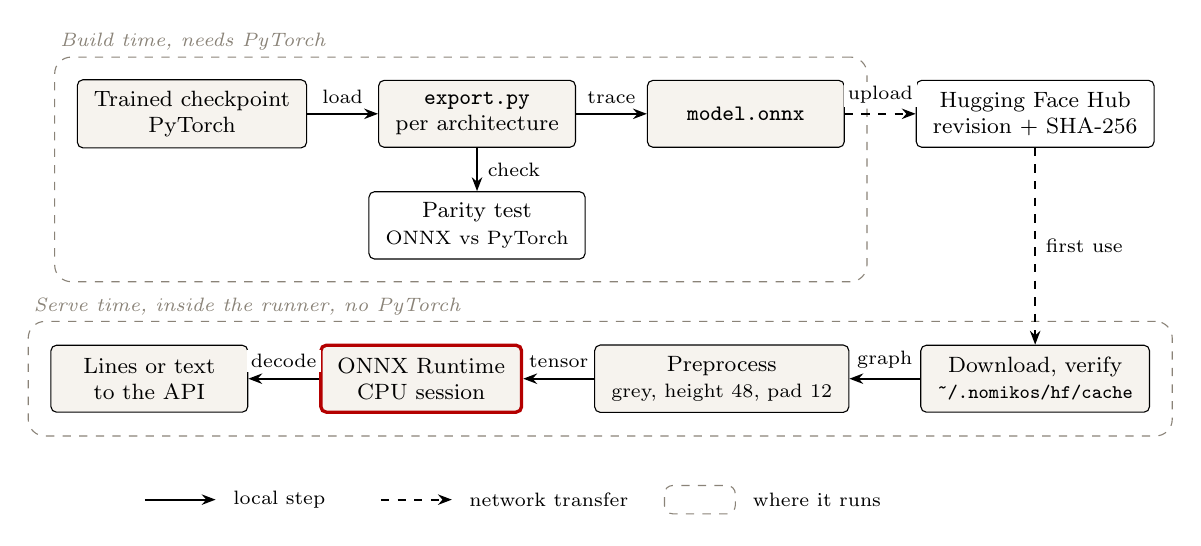
\begin{tikzpicture}[node distance=0.55cm and 0.9cm]
  \node[box] (ckpt) {Trained checkpoint\\PyTorch};
  \node[box, right=of ckpt] (exp) {\texttt{export.py}\\per architecture};
  \node[box, right=of exp] (onnx) {\texttt{model.onnx}};
  \node[store, right=of onnx] (hub) {Hugging Face Hub\\revision + SHA-256};
  \node[box, below=2.5cm of hub] (cache) {Download, verify\\\scriptsize\texttt{\textasciitilde/.nomikos/hf/cache}};
  \node[box, left=of cache] (pre) {Preprocess\\\scriptsize grey, height 48, pad 12};
  \node[box, left=of pre, draw=accent, very thick] (ort) {ONNX Runtime\\CPU session};
  \node[box, left=of ort] (out) {Lines or text\\to the API};
  \node[box, below=0.55cm of exp, fill=white] (par) {Parity test\\\scriptsize ONNX vs PyTorch};

  \begin{scope}[on background layer]
    \node[group, fit=(ckpt)(exp)(onnx)(par)] (gbuild) {};
    \node[group, fit=(out)(ort)(pre)(cache)] (gserve) {};
  \end{scope}
  \node[glabel] at (gbuild.north west) {Build time, needs PyTorch};
  \node[glabel] at (gserve.north west) {Serve time, inside the runner, no PyTorch};

  \draw[run] (ckpt) -- node[lab, above=2pt] {load} (exp);
  \draw[run] (exp) -- node[lab, above=2pt] {trace} (onnx);
  \draw[art] (onnx) -- node[lab, above=2pt] {upload} (hub);
  \draw[run] (exp) -- node[lab, right=2pt] {check} (par);
  \draw[art] (hub) -- node[lab, right=2pt] {first use} (cache);
  \draw[run] (cache) -- node[lab, above=2pt] {graph} (pre);
  \draw[run] (pre) -- node[lab, above=2pt] {tensor} (ort);
  \draw[run] (ort) -- node[lab, above=2pt] {decode} (out);

  \begin{scope}[shift={(-0.6,-4.9)}]
    \draw[run] (0,0) -- (0.9,0); \node[key] at (1.0,0) {local step};
    \draw[art] (3.0,0) -- (3.9,0); \node[key] at (4.0,0) {network transfer};
    \draw[groupline, dashed, rounded corners=3pt] (6.6,-0.18) rectangle (7.5,0.18);
    \node[key] at (7.6,0) {where it runs};
  \end{scope}
\end{tikzpicture}}
\caption{From a trained model to a served one. The registry pins each model to a Hub revision and a file hash, so every runner loads the same bytes.}
\label{fig:onnx}
\end{figure}

Adding a model follows the same path: export it and pass the parity test, publish it to the Hub, add an entry with its revision and file hash to the registry, insert a row in the model catalog table so it appears in the editor's model picker, deploy the API, and release a new runner so runners carry the entry. Each runner downloads the weights on first use.

\choice{The API contract is generated.} A script exports the OpenAPI description of the FastAPI app (115 operations), and openapi-typescript turns it into TypeScript types for the frontend. A pre-commit hook regenerates both, and CI fails if they drift. If the backend drops a field, the frontend stops compiling, so the two sides cannot go out of sync on \texttt{main}.

\section{Data model}\label{sec:data}

\choice{Model output is never overwritten.} Each segmentation run is stored once in \code{segmentation_runs} as JSON with the model name and version, and never updated. Human edits go to the live lines and to a separate \code{ground_truth} transcription layer. Comparing the two shows exactly what a person fixed, including lines they deleted, and that difference is the training data. Overwriting the model output in place would save space but lose that record, so we keep every run and accept that storage only grows.

\begin{figure}[!ht]
\centering
\resizebox{0.7\linewidth}{!}{%
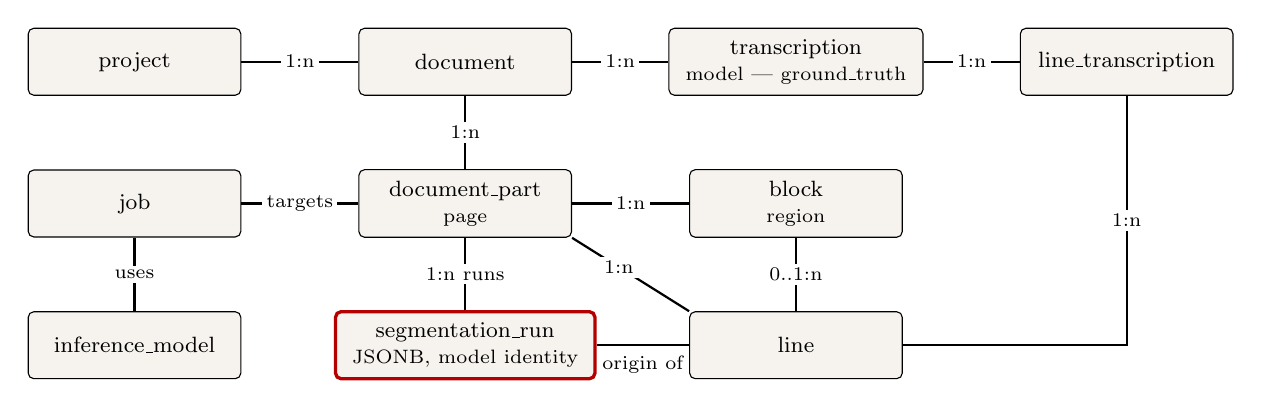
\begin{tikzpicture}[ent/.style={box, minimum width=2.7cm}, rel/.style={thick}]
  \node[ent] (proj) at (0,0) {project};
  \node[ent] (doc) at (4.2,0) {document};
  \node[ent] (tr) at (8.4,0) {transcription\\\scriptsize model | ground\_truth};
  \node[ent] (lt) at (12.6,0) {line\_transcription};
  \node[ent] (job) at (0,-1.8) {job};
  \node[ent] (page) at (4.2,-1.8) {document\_part\\\scriptsize page};
  \node[ent] (block) at (8.4,-1.8) {block\\\scriptsize region};
  \node[ent] (model) at (0,-3.6) {inference\_model};
  \node[ent, draw=accent, very thick] (run) at (4.2,-3.6) {segmentation\_run\\\scriptsize JSONB, model identity};
  \node[ent] (line) at (8.4,-3.6) {line};

  \draw[rel] (proj) -- node[lab] {1:n} (doc);
  \draw[rel] (doc) -- node[lab] {1:n} (tr);
  \draw[rel] (tr) -- node[lab] {1:n} (lt);
  \draw[rel] (doc) -- node[lab] {1:n} (page);
  \draw[rel] (job) -- node[lab] {targets} (page);
  \draw[rel] (job) -- node[lab] {uses} (model);
  \draw[rel] (page) -- node[lab] {1:n} (block);
  \draw[rel] (page) -- node[lab] {1:n runs} (run);
  \draw[rel] (page.south east) -- node[lab, pos=0.4] {1:n} (line.north west);
  \draw[rel] (block) -- node[lab] {0..1:n} (line);
  \draw[rel] (run) -- node[lab, below=2pt] {origin of} (line);
  \draw[rel] (line.east) -| node[lab, pos=0.75] {1:n} (lt.south);
\end{tikzpicture}}
\caption{Core entities; users, sharing and history tables are left out. The outlined entity is written once and never updated.}
\label{fig:er}
\end{figure}

A project holds documents, a document holds pages, and a page holds regions and lines (Figure~\ref{fig:er}). Text does not live on the line. It lives in \code{line_transcription}, one row per line and per transcription layer, so the model's text and the human's text sit side by side. Every model-proposed line points back to the segmentation run that proposed it, and the run keeps the model identity as text, so the history survives even if the job or the catalog row is deleted. A job row carries its own claim state (who holds it, how often it was claimed, when it last reported), which is all the queue needs.

\section{Security}

\begin{figure}[!ht]
\centering
\resizebox{0.86\linewidth}{!}{%
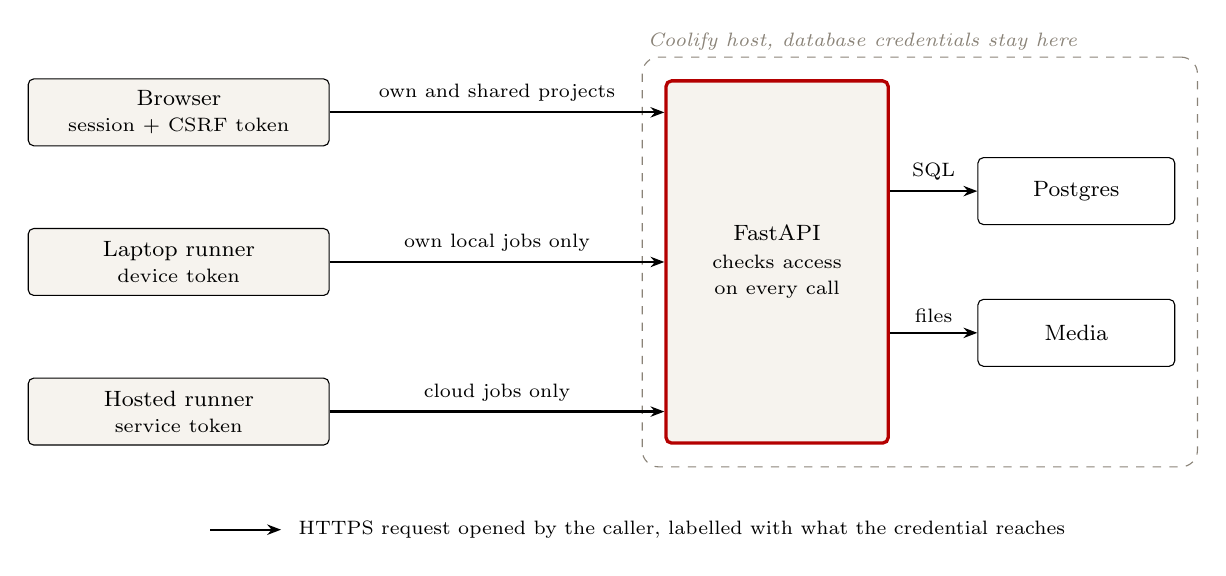
\begin{tikzpicture}
  \node[box, text width=3.4cm, align=center] (br) at (-1,0) {Browser\\\scriptsize session + CSRF token};
  \node[box, text width=3.4cm, align=center] (la) at (-1,-1.9) {Laptop runner\\\scriptsize device token};
  \node[box, text width=3.4cm, align=center] (ha) at (-1,-3.8) {Hosted runner\\\scriptsize service token};
  \node[box, draw=accent, very thick, minimum height=4.6cm, text width=2.4cm, align=center] (api) at (6.6,-1.9) {FastAPI\\[2pt]\scriptsize checks access\\\scriptsize on every call};
  \node[store] (pg) at (10.4,-1.0) {Postgres};
  \node[store] (md) at (10.4,-2.8) {Media};
  \draw[run] (br.east) -- node[lab, above=2pt] {own and shared projects} (br.east -| api.west);
  \draw[run] (la.east) -- node[lab, above=2pt] {own local jobs only} (la.east -| api.west);
  \draw[run] (ha.east) -- node[lab, above=2pt] {cloud jobs only} (ha.east -| api.west);
  \draw[run] (api.east |- pg) -- node[lab, above=2pt] {SQL} (pg);
  \draw[run] (api.east |- md) -- node[lab, above=2pt] {files} (md);
  \begin{scope}[on background layer]
    \node[group, fit=(api)(pg)(md)] (gs) {};
  \end{scope}
  \node[glabel] at (gs.north west) {Coolify host, database credentials stay here};
  \begin{scope}[shift={(-0.6,-5.3)}]
    \draw[run] (0,0) -- (0.9,0); \node[key] at (1.0,0) {HTTPS request opened by the caller, labelled with what the credential reaches};
  \end{scope}
\end{tikzpicture}}
\caption{Three credentials, one entry point. Each caller gets only the rights its token carries, and runners only ever open connections to the API, so no inbound port is needed on a laptop or behind a university firewall. Nothing outside the host holds a database password.}
\label{fig:security}
\end{figure}

Figure~\ref{fig:security} shows who can reach what. The browser never talks to Postgres or storage directly, and images come through short-lived signed URLs. We chose not to use Postgres row-level security, so FastAPI checks access before every query. All authorisation lives in one layer, which is easy to audit but means every new route has to remember the check. FastAPI also owns authentication: password hashes, JWT access tokens with rotating sessions, CSRF checks and rate-limited logins. A laptop runner never sees a password. It pairs once through a flow modelled on the OAuth device authorization grant (\href{https://www.rfc-editor.org/rfc/rfc8628}{RFC 8628}): the runner opens the browser, the signed-in user approves the device, and the runner receives a device token that it sends in its own header. That token can claim only its owner's local jobs.

The completion callback is narrowed in the same way. The API records which runner holds each job in \code{jobs.claimed_by} and accepts a result only from that runner, so one paired laptop cannot complete or fail anyone else's work. Runners get only inference and callback credentials, never database or JWT secrets. Before loading a model, a runner checks the file against the SHA-256 hash pinned in the registry.

\section{Usage and quality}

Table~\ref{tab:usage} gives the numbers from the admin dashboard for the 90 days up to 30 October 2026. They show that the platform is used, not yet how much faster transcription has become: we have not measured the ten-times target.
% TODO(usage table): add a local vs hosted split of jobs once the read-only production query has been run.

\begin{table}[ht]
\centering
\small
\begin{tabular}{@{}l r@{}}
\toprule
Measure & Value \\
\midrule
Accounts (four of them test or service accounts) & 18 \\
Jobs run & 1,070 \\
\quad transcriptions & 876 \\
\quad segmentations & 194 \\
Median transcription time per page, by model & 2.5 to 3.3\,s \\
Median segmentation time per page, current segmenters & 14 to 36\,s \\
\bottomrule
\end{tabular}
\caption{Usage over 90 days. Times run from job creation to completion.}
\label{tab:usage}
\end{table}

CI on GitHub Actions runs type checks, linting and tests for both frontend and backend, integration tests against a real Postgres 16, a nightly run on real model weights and the API contract check. Secret scanning, dependency audits and container scans run alongside, and the runner is released to PyPI through trusted publishing. The backend has 889 unit tests and 298 integration tests, of which 170 need a running Postgres. A local run of the unit tests alone covers 56\,\% of statements and branches in the backend and the runner. An admin dashboard shows users, jobs per model with success rate and median duration, request timings per route, and the failure reports and feedback that users send.

\section{Limits and next steps}

Two weaknesses matter today:
\begin{itemize}
  \item \textbf{Schema changes by hand.} Alembic holds the revision history, but the production container never runs it. Before Coolify deploys, a release script applies dated SQL by hand and checks the recorded Alembic version; running migrations automatically would be safer.
  \item \textbf{One host.} The API, Postgres and the media directory share one Coolify host, so it is a single point of failure. Backups leave the host, so the data survives a lost machine, but the service does not survive an outage. The first step is to give Postgres its own host or a managed service.
\end{itemize}



\end{document}
